\documentclass[12pt]{article}
\usepackage[utf8]{inputenc}
\usepackage[T1]{fontenc}
\usepackage[spanish]{babel}
\usepackage{graphicx}
\usepackage{xcolor}
\usepackage{lmodern}
\pdfpagewidth=420mm
\pdfpageheight=297mm
\setlength{\paperwidth}{420mm}
\setlength{\paperheight}{297mm}
\setlength{\textwidth}{395mm}
\setlength{\textheight}{272mm}
\setlength{\oddsidemargin}{-1in}
\addtolength{\oddsidemargin}{12.5mm}
\setlength{\topmargin}{-1in}
\addtolength{\topmargin}{12.5mm}
\setlength{\headheight}{0pt}
\setlength{\headsep}{0pt}
\setlength{\parindent}{0pt}
\setlength{\parskip}{0.2em}
\pagestyle{empty}

\definecolor{azulubu}{HTML}{172033}
\definecolor{azulazure}{HTML}{0067B8}
\definecolor{fondoclaro}{HTML}{F5F7FA}
\definecolor{linea}{HTML}{D8DEE7}

\newcommand{\bloque}[2]{%
  \colorbox{fondoclaro}{%
    \begin{minipage}[t]{0.965\linewidth}
      \vspace{0.25cm}
      {\Large\bfseries\color{azulazure} #1}\par
      \vspace{0.12cm}
      #2
      \vspace{0.25cm}
    \end{minipage}}}

\begin{document}
\begin{center}
  
\includegraphics[width=0.34\textwidth,height=1.7cm,keepaspectratio]{../../memoria/img/cabecera.png}

  \vspace{0.08cm}
  {\fontsize{22}{25}\selectfont\bfseries\color{azulubu}
  Cloud Computing: análisis, diseño y despliegue de un servicio empresarial seguro en Microsoft Azure\par}
  \vspace{0.08cm}
  {\large Karima Drafli Rico \hspace{1.2cm} Tutor: José Ignacio Santos Martín}
\end{center}

\vspace{0.2cm}
\small
\begin{minipage}[t]{0.25\textwidth}
  \bloque{Problema empresarial}{
    Las solicitudes internas de TI suelen llegar por canales dispersos, con prioridades poco homogéneas, credenciales expuestas y escasa trazabilidad. Esto dificulta asignar responsables, controlar plazos y justificar cada decisión.
  }

  \vspace{0.35cm}
  \bloque{Objetivo}{
    Diseñar y validar una plataforma cloud que automatice el ciclo completo de una solicitud: registro, clasificación, aprobación, asignación, escalado, seguimiento del SLA, cierre y valoración.
  }

  \vspace{0.35cm}
  \bloque{Aportación}{
    \begin{itemize}
      \setlength{\itemsep}{0.14cm}
      \item Catálogo de servicios, activos y criticidad.
      \item Clasificador ligero, explicable y reproducible.
      \item Aprobación de accesos y cambios sensibles.
      \item Centro operativo con alertas, SLA e informes.
    \end{itemize}
  }
\end{minipage}
\hfill
\begin{minipage}[t]{0.72\textwidth}
  \bloque{Arquitectura desplegada y verificable}{
    \centering
    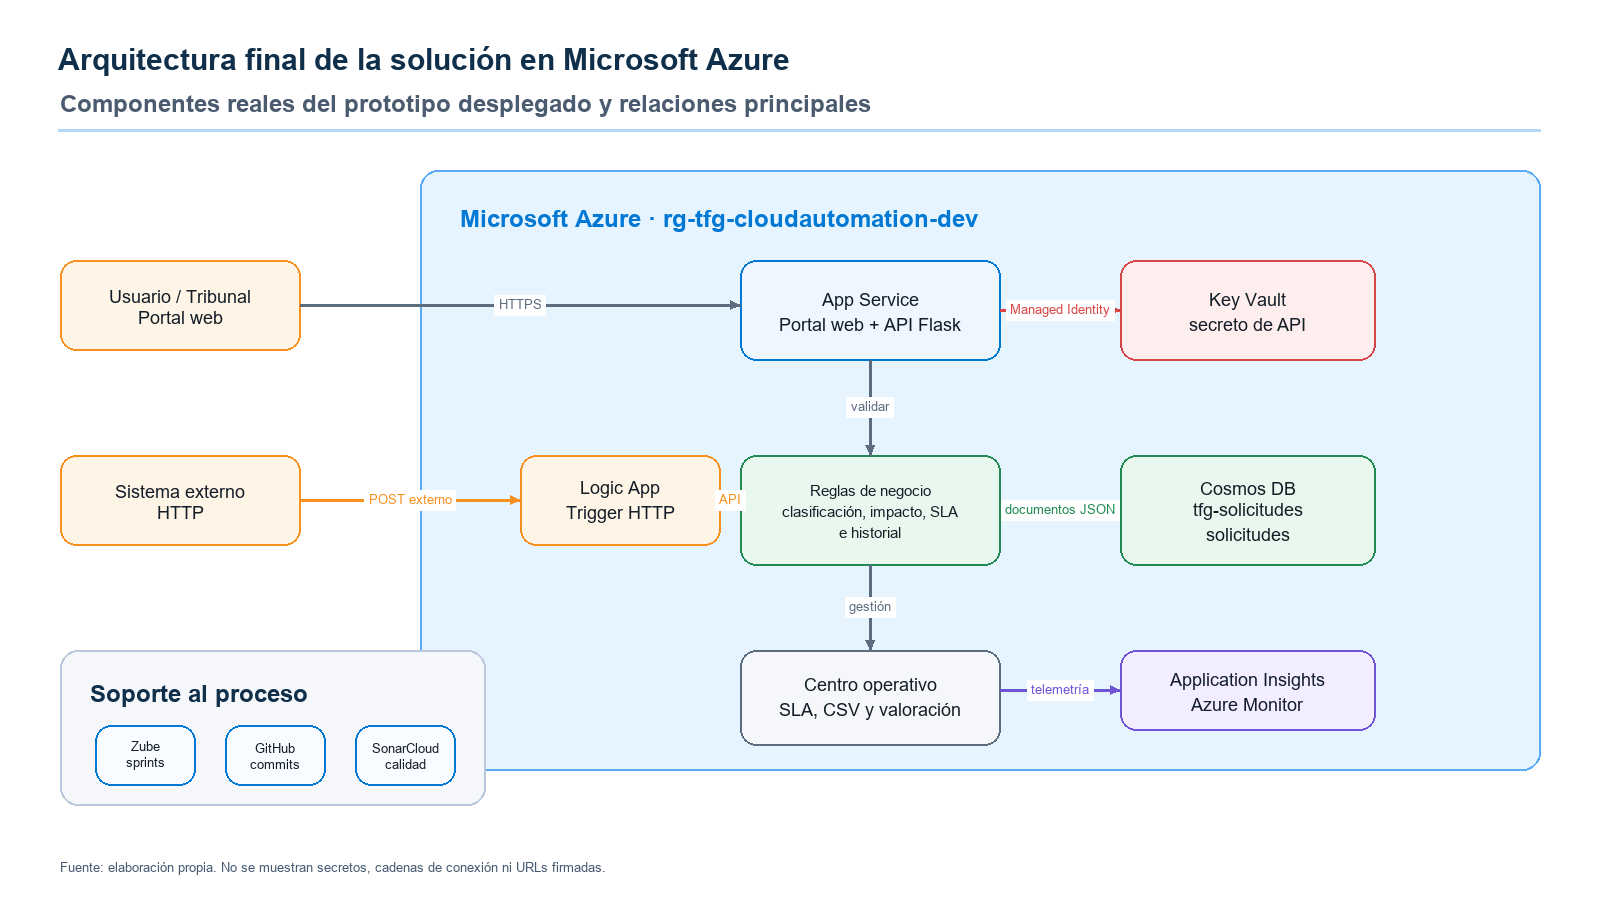
\includegraphics[width=0.97\linewidth,height=6.3cm,keepaspectratio]{../../memoria/img/arquitectura_final_azure.png}
  }

  \vspace{0.35cm}
  \begin{minipage}[t]{0.60\linewidth}
    \bloque{Producto funcional}{
      \centering
      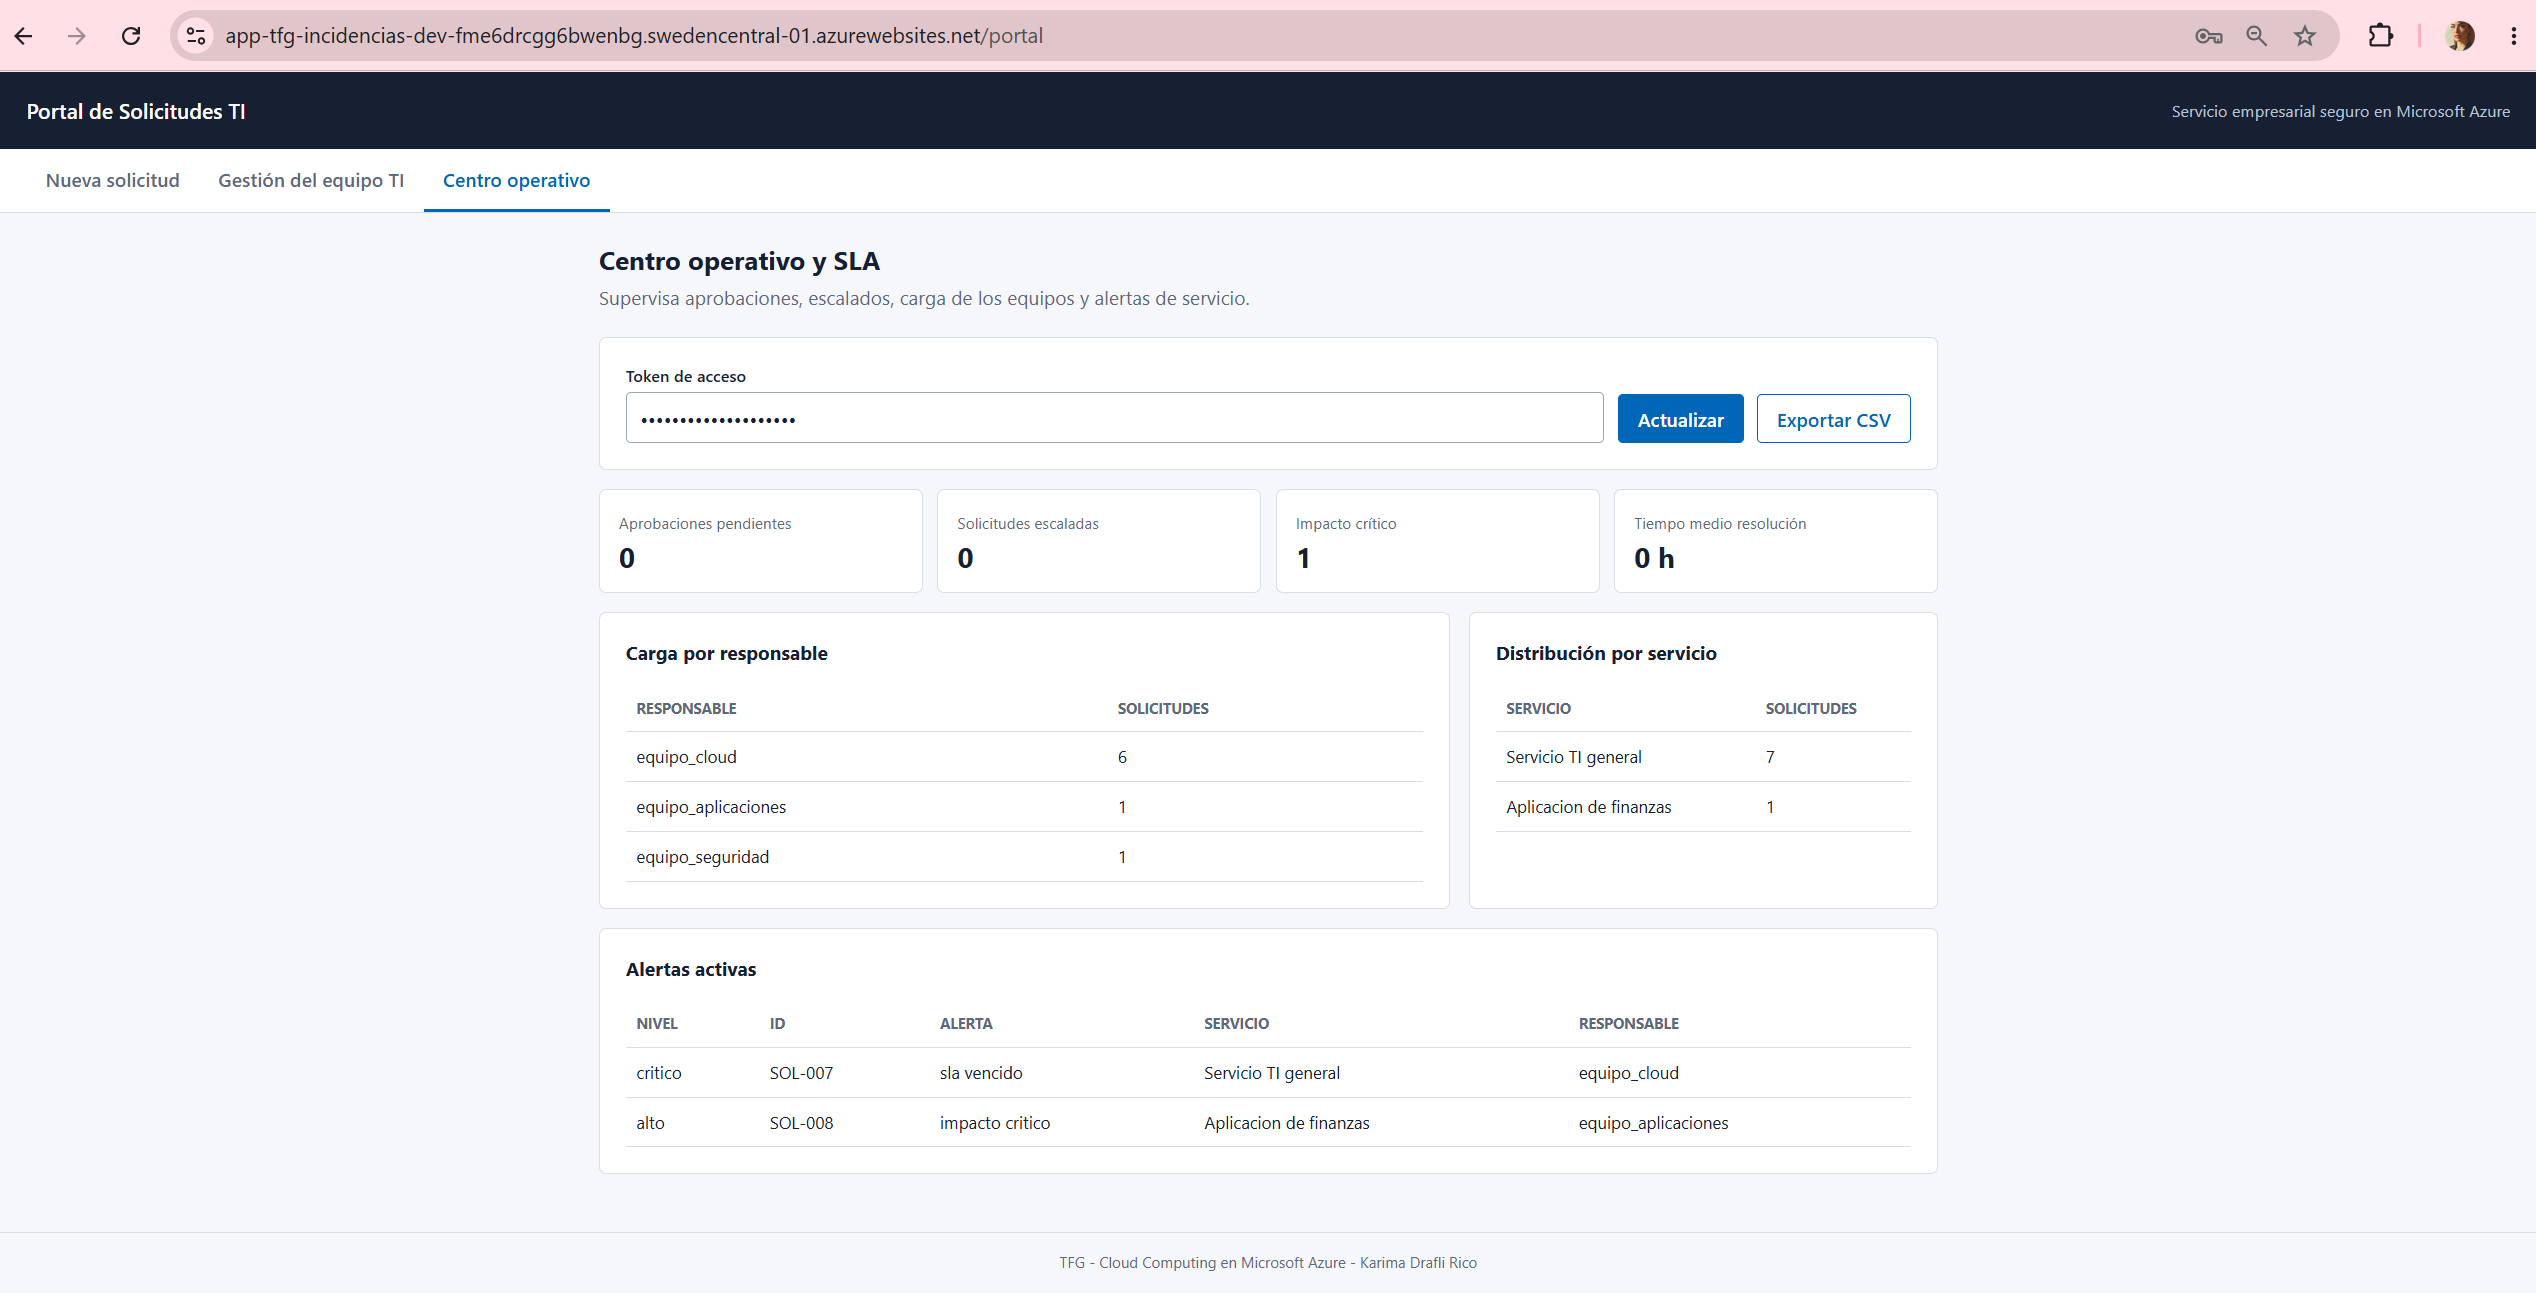
\includegraphics[width=0.98\linewidth,height=4.6cm,keepaspectratio]{../../memoria/img/portal-centro-operativo-sla.png}

      \small El portal permite registrar solicitudes y al equipo TI gestionar aprobaciones, responsables, escalados, vencimientos y exportaciones.
    }
  \end{minipage}
  \hfill
  \begin{minipage}[t]{0.37\linewidth}
    \bloque{Validación y resultados}{
          \begin{itemize}
            \setlength{\itemsep}{0.2cm}
        \item 27 pruebas automáticas superadas.
        \item Quality Gate de SonarCloud aprobado.
        \item Despliegue real en Azure App Service.
        \item Cosmos DB documental y Key Vault.
        \item Managed Identity sin credenciales Azure en código.
        \item Logic App como canal de integración HTTP.
        \item Application Insights y Azure Monitor.
        \item Cinco sprints gestionados en Zube.
      \end{itemize}
    }

    \vspace{0.35cm}
    \bloque{Conclusión}{
      El prototipo demuestra que un proceso interno puede automatizarse con servicios gestionados de Azure manteniendo seguridad, trazabilidad y capacidad de evaluación. La solución es extensible, aunque una implantación productiva requeriría identidad corporativa y autenticación corporativa avanzada y gobierno de datos.
    }
  \end{minipage}
\end{minipage}

\vfill
\begin{center}
  \footnotesize\color{azulubu}\bfseries
  Repositorio, portal, documentación OpenAPI, planificación y calidad enlazados desde GitHub:
  github.com/karimadrico/tfg-azure-servicio-empresarial-seguro
\end{center}
\end{document}
